\documentclass[conference]{IEEEtran}
\usepackage[T1]{fontenc}
\usepackage[utf8]{inputenc}

\usepackage{fullpage}
\usepackage[french]{babel}
\usepackage{graphicx}
\usepackage{todonotes}

\title{PROJ: DeepVoice}

\author{Remi Hutin, Rémy Sun, Raphael Truffet \\
  \{Remi.Hutin, Remy.Sun, Raphael.Truffet\}@ens-rennes.fr \\
  Département informatique, ENS Rennes \\
  Campus de Ker lann, Bruz, France
\and
  Guillaume Gravier \\
  guig@guig.fr\\
  Medialink project, INRIA \\
  Campus de Beaulieu, Rennes, France
 }
\begin{document}

\maketitle

\section{Introduction}

\section{Sound signals}

\subsection{Cepstral analysis}

The speech signal of a locutor is hardly suitable for statistical modeling or the calculation of a distance.
In order to obtain a representation which is more compact and less redundant, we use a cepstral representation of the speech.

The cepstrum of a signal $x(t)$ is defined by :

$$C(x(t)) = \mathcal{F}^{-1}(\ln(|\mathcal{F}(x(t))|)$$

where $\mathcal{F}$ is the Fourier transform.



We can analyze a signal locally by applying a window, whose duration is shorter than the signal. Then, we exctract a vector of cepstral coefficents of this part of signal. We repeat it for several windows, until the end of the signal is reached.

\todo[inline]{distance}


\subsection{Gaussian Mixture Model (GMM)}

A Gaussian Mixture Model (GMM) is probabilistic model used to approximate a distribution of random variables as a sum of normal distributions. Here, we are trying to represent the distribution of the cepstral vectors of a signal as a sum of normal distributions using a reference model.



\subsection{Supervectors and i-vectors}

\subsection{Previous works}

\section{Use of neuronal networks}

\subsection{Formal neuron}

\paragraph{Neuron?}
A neuron can be thought of as a function which takes an $n$-dimensional vector $A$ as input and returns a scalar $e$ as output. This function typically has two internal parameters which are a bias $b$ and a weight-matrix $W$. The function starts by calculating $WA+b$ before using a non-linear activation function (such as sigmoid or tanh): $e=f(WA+b)$.

\paragraph{Adjusting the function}

Our endgoal is to have the neuron, and by extension the neural network, perform
a certain task. The formal neuron \og learns\fg by adjusting its function to perform better on
this designated task. For simplicity's sake, we will first explain how this
process - called \og backpropagation\fg{} - works with a single neuron.

For instance, suppose we have a bi-dimensional vector given as input and that we
want our neuron to return 1 if its two coordinates are the identical and -1 if
it is not. A natural way to evaluate how accurate our neuron is by looking at the
distance between its output $e$ and the desired result r : d(e)=|e-r|.

We want to modify our neuron/function to minimize this distance. That means
changing $e$, typically by gradient descent on function $d$ derivative. Here,
$\frac{\partial d}{\partial e} = r-e$, which means we want to \og move\fg{} $e$ in this
direction. To this end, we modify our function's two internal parameters $W$ and
$b$. $e$, and by extension $d$, can actually be seen as a function of those two
parameters: $d(W,b)=|e(W,b)-r|$. Therefore $\frac{\partial d}{\partial W}
   = \frac{\partial d}{\partial e}\frac{\partial e}{\partial W}$,
$\frac{\partial d}{\partial b}
   = \frac{\partial d}{\partial e}\frac{\partial e}{\partial b}$. We then only
   need to compute new internal parameters $W'$ and $b'$ with 

\begin{equation}
     W'=W + s\frac{\partial d}{\partial W}=W-s\frac{\partial d}{\partial e}\frac{\partial e}{\partial W}
\end{equation}

\begin{equation}
     b'=b + s\frac{\partial d}{\partial b}=b-s\frac{\partial d}{\partial e}\frac{\partial e}{\partial b}
\end{equation}

What we just demonstrated was a simple backpropagation algorithm called gradient
descent. This method is deeply flawed, but most state of the art backpropagation
methods find their origins in this humble algorithm.

\paragraph{Neuronal network?}

Typically, a neural \textbf{network} is made up of more than a single neuron. A
neural layer refers to multiple neurons working on the same input (or parts of
the same input) and producing an output that can be construed as some form of
concatenation of their respective outputs. This output can be in turn regarded
as an alternate representation of the input. Backpropagation for each neuron
works the same way as it would if it were the only neuron calculating.

The notion of \textbf{deep} learning comes from the fact that the alternate
reprensentation computed by one layer $A$ can be fed as input to another layer $B$.
This allows networks to infer multiple levels of representation, same as one
first processes simple geometrical forms before recognizing more complex
compositions. Backpropagation is straight-forwardly computed on layer $B$. It is
computed on layer $A$ by looking at $\frac{\partial d}{\partial input_B}$
instead of $\frac{\partial d}{\partial e}$
\subsection{Autoencoders}

An autoencoder is a neuronal network with a particular architecture which is defined below.

\paragraph{A default goal}
Basically, in order to learn a neuronal network, we need to affect to each input of the learning set a label, that is the output we want to enclose, the desired result. However, autoencoders bypass this need by defaulting to an objective that does not require additional information on the input. In fact, the desired result is the input itself.

\paragraph{Structure}
A neuronal network that tries to reconstruct the input may learn the identity. But an autoencoder has a structure the makes it impossible. In fact, an autoencoder has at least one hidden layer that is smaller than the input. So an autoencoder can be decomposed as an encoder that transform the input to a smaller represatation, called latent representation or code, and a decoder that reconstruct the input from the latent representation.

\begin{figure}[!h]
    \centering
    \caption{Structure of an autoencoder}
    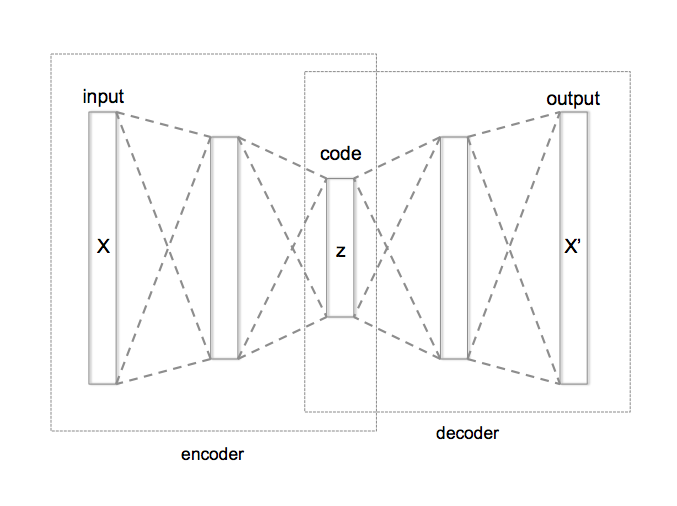
\includegraphics[width=7cm]{Autoencoder_structure.png}
    \label{autoencoder_structure}
\end{figure}


\paragraph{Why use autoencoders?}

Autoencoders can be used for denoising, using corrupted data as input and the original data as objective.

Autoencoders may also be very useful to learn a representation. In fact, the latent represention contains enough information to reconstruct the data.

In our context, autoencoders could be used to find a representation of a speaker, by giving to the autoencoder an i-vector from a speaker as input, and an another i-vector from the same speaker as objective. This idea is based on considerating the withoin-speaker variability as a noise, and using a denoising autoencoder. Repeating this with several pairs of i-vectors, we may learn a representation of the speaker. 



\subsection{Tied weight autoencoder}

\paragraph{Architecture}
[Explanation]

\paragraph{Good results}
[Vedran's paper?]

\section{Method}

As explained earlier, supervectors computed from Gaussian Mixture Models provide
useful features of a given signal. i-vectors have built upon this representation
to extract a more compact reprensentation that better reprensent the
specificities of the signal.

One task that naturally comes to mind is deciding whether two signals have been
said by the same person. Unfortunately, computing euclidian distance between the signals'
respective supervector or i-vector does not yield satisfactory results.
Therefore, we will use neural networks to extract an intermediate representation
of each signal that might be better suited to this particular problem.

\subsection{Prospective methodology}

\paragraph{Phasing out non-speaker dependant noise}

In order to extract a representation of supervectors that makes speaker
dependent features of the given signal more salient, we use a model derived from
the design of a denoising autoencoder. Indeed, we have no need for any
information pertaining to what is actually being said or what kind of microphone
was used: this is all noise to us. Therefore, if two supervectors originate from
the same speaker, it seems reasonnable to think of them as the same original \og
speaker\fg{} sound vector which has polluted by non-speaker dependant noise.

The latent representation thusly extracted should present salient features
specific to the studied speaker. An autoencoder trained that way could allow for
a sort of projection that we wish to study.

\paragraph{Prospective general model}

We will therefore train an autoencoder on supervectors. Given good results of
[Vedran's paper], we will tie all but the extreme weights to reflect the
symmetrical nature of the task at hand.

\subsection{Preliminary results}

In light of the difficulties inherent to the training of large neural networks,
a preliminary study on a small dataset has been conducted.

\subsubsection{Dataset}

\paragraph{Processing raw data}

15311 audio signals were extracted from BFMTV's various programs and labeled
with the name of their respective speaker. Those soundfiles were then processed
into 15311 supervectors of length 9311 (?) with the \texttt{AudioSeg} tool.
We then create 1800000 pairs of supervectors that originate from the same
speaker.

\paragraph{Input}

For each computed pair, we feed both of its suervectors to the neural network as
input. Therefore, we train the network on 3 600 000 supervectors of size 9311.

\paragraph{Output and task}

The neural network outputs a vector of size 9311 that we try to match as closely
as possible to the supervector the original input was paired with.




\end{document}
